\chapter{Shapelet问题描述及算法}
\label{cha:chap02}
这一部分主要介绍了Shapelet相关定义,对于距离测度方法进行了分析和比较,介绍了Shapelet计算流程,对于Shapelet通用算法进行了分析。
\section{Shapelet相关定义}
\label{cha:chap02:def}
这一部分介绍Shapelet的相关定义\cite{ye2009time},这些定义是理解Shapelet流程的前提。

\begin{definition}
	数据集的表示:对于一个时间序列数据集$D$,和其他数据集一样,都是由输入(特征向量)与输出(类标)组成,数据集通常表示为公式~\ref{equ:chap2:Dataset}形式。其中$T_i$是一个时间序列,$y_i$是其类标。
\end{definition}
\begin{equation}
\label{equ:chap2:Dataset}
D = \left\lbrace (T_1,y_1),(T_2,y_2),\cdots (T_N,y_N)\right\rbrace 
\end{equation}

\begin{definition}
	时间序列$T_i=t_1,\cdots,t_L$是由$L$个实数组成的有序集合。$t_1,\cdots,t_L$是按时间顺序排列并且具有相同的时间间隔。时间序列$T_i$的长度可以用$|T_i|$表示。
\end{definition}

\begin{definition}
\label{def:chap02:Subsequence}
	子序列($Subsequence,S$),对于长度为$L$的时间序列$T_i$,对于任何一个子序列可以由两个参数( 起始位置$st$和子序列长度$len$)确定唯一的子序列$T_{i,st}^{len}(s.t.\quad st+len <= L)$。时间序列$T_i$的子序列集合可以通过$Subset(T_i)$表示,$Subset(T_i)$集合大小为$\frac{L(L+1)}{2}$(这里不包括长度为0的时间序列)。数据$D$的子序列结合用$SubSet(D)$表示,数据集$D$是$N$个长度$L$的时间序列,则$SubSet(D)$的集合大小为$\frac{NL(L+1)}{2}$。

\end{definition}

\begin{definition}
	时间序列之间的距离$Dist(A,B)$,用于表示具有相同长度的时间(子)序列$A$和时间(子)序列$B$的空间距离,作为距离,满足对称性、非负性、三角不等式形式的,就可以满足$Dist(A,B)$的要求,原始算法使用欧式距离($Euclidean\quad distance$),这里可以扩展到广义距离,可以包括曼哈顿距离,欧氏距离,$DTW$距离等。
\end{definition}

\begin{definition}
\label{def:chap2:SubDist}
	时间子序列$S$到时间序列$T_j$之间的距离(必须满足$|S|<=|T_j|$),是所有$T_j$序列中长度为$S$的子序列与$S$距离的最小值,如~\ref{equ:chap2:SubDist}。子序列$S$和数据集$D$的所有时间序列取距离,可以获得一个$(SubDist(S,T_j),y_j)$的集合$\mathcal{F}$,如~\ref{equ:chap2:SubDistSet}。
\end{definition}
\begin{equation}
\label{equ:chap2:SubDist}
	SubDist(S,T_j) = \min (Dist(S,T_{j,u}^{|S|})),u=1,\cdots,|T_j|-|S|+1,s.t. |S| <= |T_j|
\end{equation}

{\color{red}{这里为$\mathcal{F}_{i,1},\mathcal{F}_{i,2}$做一下定义,为4.4服务一下}}

{\color{red}{数据集$D$到$S$相对数据集$D$距离-类标对集合$\mathcal{F}$和dist,label一块在这解释一下}}



\begin{equation}
\label{equ:chap2:SubDistSet}
	\mathcal{F} = \left\lbrace (SubDist(S,T_1),y_1),(SubDist(S,T_2),y_2),\cdots,(SubDist(S,T_N),y_N) \right\rbrace 
\end{equation}

\begin{definition}
	信息增益,根据特征$A$将训练数据集$D$划分为$M$个子集$D_1,D_2,\cdots,D_M$,$A$对于数据集$D$的信息增益$g(D,A)$为数据集D的熵$H(D)$和$A$给定条件下经验条件熵$H(D|A)$之差,即~\ref{equ:chap2:Infogain}
\end{definition}
\begin{equation}
\label{equ:chap2:Infogain}
g(D,A) = H(D) - H(D|A) = H(D) - \sum_{i=1}^{M}\frac{|D_i|}{|D|}H(D_i|A)
\end{equation}
	对于子序列$S$与数据集$D$中每一个时间序列$T(T\in D)$的距离$SubDist(S,T)$,$SubDist(S,T)$分布在$(0,\infty)$,如图~\ref{fig:SubDist},子序列$S$和分割点$d_{th}$共同作为特征$(S,d_{th})$将数据集$D$分为$D_1 = \left\lbrace T,SubDist(S,T)<d_{th} \& T\in D\right\rbrace $和$D_2 = \left\lbrace T,SubDist(S,T) \geq d_{th}\& T\in D\right\rbrace$两部分。子序列-分割点特征$(S,d_{th})$相对数据集的信息增益为数据集$D$的熵减去子集$D_1$和子集$D_2$的权重和,如~\ref{equ:chap2:Infogain2}
\begin{equation}
\label{equ:chap2:Infogain2}
g(D,(S,d_{th})) =H(D)-H(D|(S,d_{th})) = H(D)-(\frac{|D_1|}{|D|}H(D_1)+\frac{|D_2|}{|D|}H(D_2))
\end{equation}
\begin{definition}
	最佳分割点:在子序列$S$下,存在一个阈值$d_{osp(S)}$,满足$g(D,(S,d_{osp(S)})) \geq g(D,(S,d_{th})),\forall d_{th}\in \mathbb{R}_{+}$,则将$d_{osp}$记为子序列$S$下的最佳分割点。
\end{definition}
\begin{figure}[H] % use float package if you want it here
	\centering
	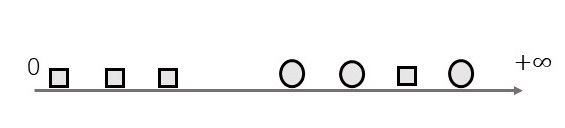
\includegraphics{SubDistDistribution.jpg}
	\caption{$SubDist(S,T),T\in D$在$(0,\infty)$的分布}
	\label{fig:SubDist}
\end{figure}

\begin{definition}
	\label{def:choose}
	$Shapelet$,对于给定数据集,对于在一个子序列$Shapelet(D)$,使$g(D,(Shapelet(D),d_{osp(Shapelet(D))})) \geq g(D,(S,d_{osp(S)})),\forall S\in SubSet(D)$
\end{definition}

从以上定义来看,时间序列中的一类存在一种模式(波形),这种模式和此类时间序列表现出较小的距离,和另一类没有这种模式的时间序列表现出较大的距离,而Shapelet算法那就是负责寻找这种模式和较小-较小距离阈值的算法。Shapelet对于所有可能子序列进行评价(~\ref{def:choose}),选出评价指标最好的子序列作为模式。


\section{距离测度方法}
\label{cha:chap02:Distance}
对于两个时间序列$A=\left\lbrace a_i\right\rbrace_{i=1}^m$和$B=\left\lbrace b_j\right\rbrace_{j=1}^n$的相似性,可以由多种方法度量,包括欧式距离( Euclidean distance,要求时间序列长度一致即$|A| = |B|$)、动态时间归整(Dynamic time warping,DTW)、最长公共子序列( Longest Common Subsequence,LCS)。其中最长公共子序比较适用于字符序列,对于实数值时间序列元素“$a_i=b_j$”进行重新定义。下面就本文用到的欧氏距离和动态时间规整进行简介。
\subsection{欧氏距离}
欧氏距离是使用最普遍的距离测度方法,是度量$M$维空间上的两个点的直线距离。将欧氏距离应用在时间(子)序列上,要求两者的长度相等。对于长度都为$M$的两个时间(子)序列$A$和$B$,两者之间的欧氏距离是两者对应元素平方和的平方根,如~\ref{equ:chap2:DistEuclid}。为了简化计算,经常使用平方和$\sum_{i=1}^{M}(A_i-B_i)^2$表示$Dist(A,B)$。

%时间序列分析和挖掘是一个广泛的研究领域,在过去的几十年中,它越来越多地用于分类,聚类,索引或检索等多种任务(参见[4]的一项调查)。 比较时间序列的一个流行的相似性度量方法是动态时间规整(Dynamic Time Warping,DTW),因为它具有处理时间偏移和变形的能力。其复杂度与时间序列长度成正比
%对于很长时间序列和/或非常大的一组时间序列,使用DTW是很困难的

\begin{equation}
\label{equ:chap2:DistEuclid}
D(A,B) = \sqrt{\sum_{i=1}^{M}(A_i-B_i)^2}
\end{equation}
\subsection{动态时间规整}


%在定义中,我们使用绝对差异来表示单个样本之间的距离。 我们的方法也适用于速度没有差异的平方差。 m×m矩阵d称为翘曲矩阵。 在变形矩阵中,每个单元格使用来自三个先前计算的邻居中的任何一个的值。 因此,如果我们回溯用于计算DTW的值(即d(m,m)),我们得到描述T和Q的最佳对齐的翘曲路径(图1)。\

%时间序列的相似性度量是时间序列数据挖掘的基础[5, 6]。时间序列由于其特定的形状特征, 使得目前常用的一些相似性度量和聚类方法失去了原有的优越性, 而几乎所有的时间序列挖掘算法都涉及到计算序列之间的相似性问题。目前,时间序列的相似性度量主要采用Lp范数(例如欧几里德距离)、动态时间弯曲距离、最长公共子序列、编辑距离、串匹配等。前两种相似性度量方法应用较为广泛。但是欧几里德距离不支持时间序列的线性漂移和时间弯曲,动态时间弯曲距离的计算量很大,不适合直接应用于海量时间序列的挖掘,从而限制了其在时间序列数据挖掘上的广泛应用。


动态时间规整\cite{muller2007dynamic}(dynamic time warping,DTW)是一种通过将一个时间序列$A$延时间轴进行非线性的延展或者压缩,目的使$A$序列和另一时间序列$B$能够很好地对齐,对齐方式如图~\ref{fig:twoplotdtw}。这种对齐方式是通过一种动态规划的算法计算获得,计算过程如图~\ref{fig:threeplotdtw},首先建立一个$|A|*|B|$的代价矩阵,通过~\ref{equ:chap2:costMatrix}递推方程获得更新之后的矩阵,从$(1,1)$到$(|A|,|B|)$存在一条从$0$累计到$D(|A|,|B|)$的叠加过程,这条路径即为规整路径,$A$和$B$在这条路径上的对应关系就是最优对齐方式,而$D(|A|,|B|)$则是用来度量$A$和$B$相似度的值。


假设有两个时间(子)序列,$C=c_1,c_2,\cdots,c_i,\cdots,c_m$和$Q=q_1,q_2,\cdots,q_j,\cdots,q_m$,$Q$和$C$之间的DTW距离用$Dist(Q,C)$来表示,$Dist(Q,C)$的计算过程如~\ref{equ:chap2:costMatrix}~\cite{sart2010accelerating}。

\begin{equation}
\label{equ:chap2:costMatrix}
\begin{array}{l}
Dist(C,Q) = d(m,m) \\ [0.3cm]
d(i,j) = |c_i-q_j|_n\footnote{n=1,2} + \min
\begin{cases}
d(i-1,j)\\
d(i,j-1)\\
d(i-1,j-1)
\end{cases}\\[0.2cm]
d(0,0)=0;d(i,0)=\infty;d(0,j)=\infty;i=1,2,\cdots,m;j=1,2,\cdots,m 
\end{array}
\end{equation}


\begin{figure}
	\begin{minipage}{0.48\textwidth}
		\centering
		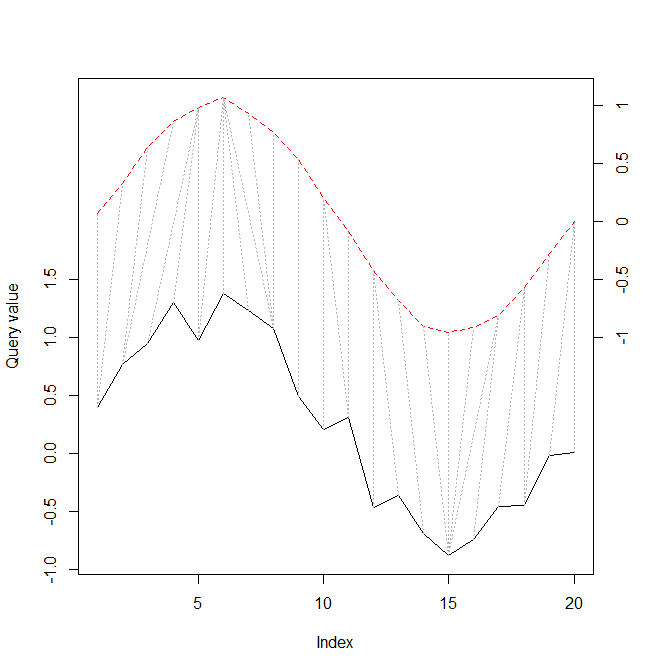
\includegraphics[height=6.2cm]{twoplotdtw.png}
		\caption{时间序列$A,B$对齐方式}
		\label{fig:twoplotdtw}
	\end{minipage}\hfill
	\begin{minipage}{0.48\textwidth}
	\centering
	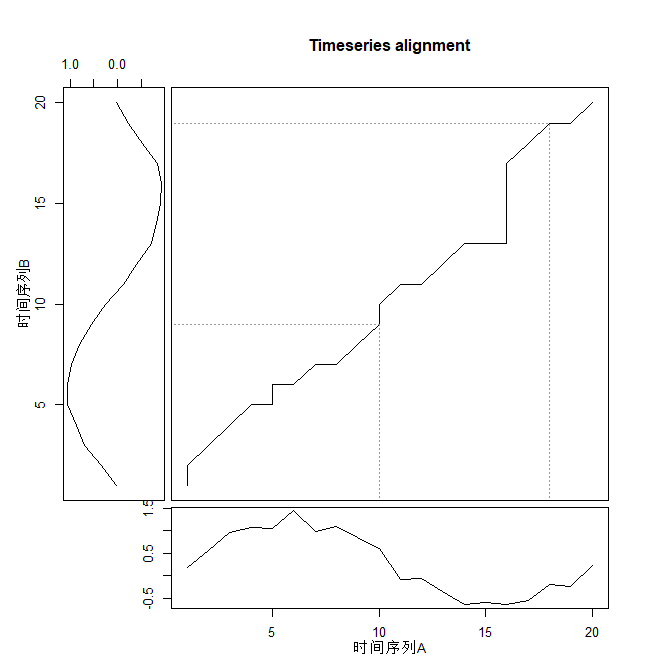
\includegraphics[width=6.2cm]{threeplotdtw.png}
	\caption{时间序列$A,B$规整路径和代价矩阵}
	\label{fig:threeplotdtw}
	\end{minipage}
\end{figure}

DTW虽然不要求时间(子)序列长度一致,但这里依然要求时间(子)序列长度一致,这里基于两个原因考虑。第一,这样对于任何一个子序列$S$与$T_i$的距离,如果不要求(子)序列长度一致,就必须计算$T_i$所有子序列和$S$的DTW距离,再在这些距离里面取最低值,这样$S$需要和$O(L^2)$个子序列计算距离,使计算的复杂度变高。第二,当不要(子)序列长度一致时,不能判断哪个时间序列更具相似性。比如有$D,E,F$三个时间序列,其中$|D|<<|E|<|F|$,$Dist(D,E) < Dist(F,E)$,但是这里不能就此认定$D$比$F$更具有相似性。

原始DTW的时间复杂度和空间复杂度都是$O(M^2)$(如果$|A|=|B|=M$)。因为$DTW$的时间和空间复杂度都比较大,有人提出了FastDTW\cite{salvador2007toward},通过将规整路径限制在一定区域内,包括$Sakoe-Chuba band$(如图~\ref{fig:Sakoe-Chuba-band})和$Itakura band$(如~\ref{fig:Itakura-band})两种方法,这两种限制区域的方式限制一些对于时间序列延展或者压缩过度以求时间序列的最佳对应的情况。相比原始DTW算法,限制区域的方法时间复杂度和空间复杂度都比较低,这种方法在牺牲很小准确率(极度延展或压缩情况)的情况下降低时间空间复杂度。$Sakoe-Chuba band$方法中的$w(w>=0)$的大小表示限制区域的宽度,当$w=0$时,限制区域为对角线;当$w=|A|$(与时间序列$A,B$长度相等)时,限制区域为真个代价矩阵,这个时候$Sakoe-Chuba band$方法等价于原始的DTW算法。本文使用$Sakoe-Chuba band$方法代替原始DTW方法作为距离测度,下文提到的DTW都是进行使用$Sakoe-Chuba band$区域限制的DTW,这里使用$DTW(A,B,w)$表示这种限制区域下的DTW,时间复杂度为$O(wM)$。
\begin{figure}
	\begin{minipage}{0.48\textwidth}
		\centering
		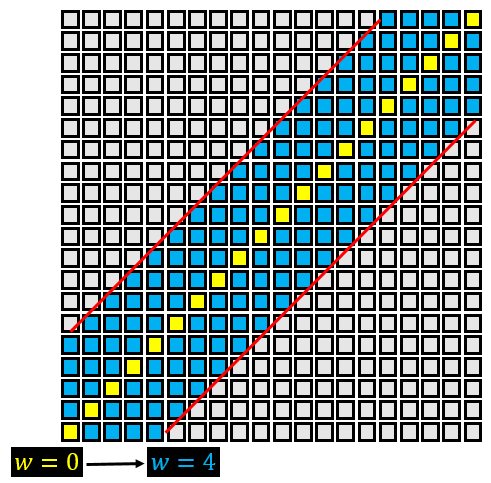
\includegraphics[height=6.2cm]{Sakoe-Chubaband.png}
		\caption{Sakoe-Chuba band}
		\label{fig:Sakoe-Chuba-band}
	\end{minipage}\hfill
	\begin{minipage}{0.48\textwidth}
		\centering
		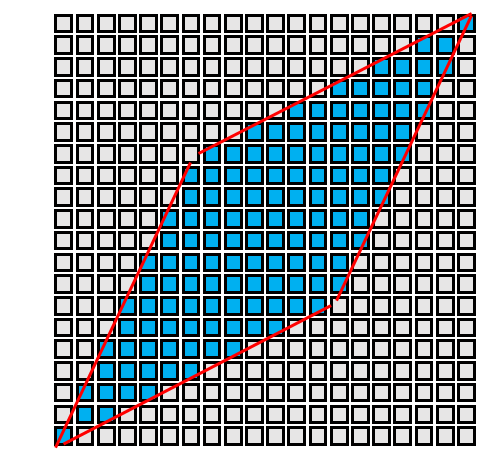
\includegraphics[width=6.3cm]{Itakuraband.png}
		\caption{Itakura band}
		\label{fig:Itakura-band}
	\end{minipage}
\end{figure}

\subsection{欧式距离与动态时间规整比较}
\label{chap02:euclid2Dtw}

%在过去的十年中,已经提出了超过一百种不同的时间序列距离测量方法[12]。 然而越来越多的经验证据表明动态时间翘曲(DTW)(包括欧几里得距离作为一种特殊情况)是跨越广泛领域的最佳测量方法[7]。
%[12]Keogh, E. J. and Kasetty, S. On the Need for Time Series Data Mining Benchmarks: A Survey and Empirical Demonstration. Data Min. Knowl. Discov. 7(4): 349-371 (2003).
%[7]
%Ding, H., Trajcevski, G., Scheuermann, P., Wang, X. and Keogh, E. Querying and Mining of Time Series Data: Experimental Comparison of Representations and Distance Measures. VLDB 2008. 

如图~\ref{fig:Sakoe-Chuba-band},当$w=0$时,DTW算法将会退化成代价矩阵的对角线,$D(i,j)$的递推方程也将变为沿对角线传递,如图~\ref{fig:Sakoe-Chuba-band}黄色部分和~\ref{equ:chap2:dtwdeg2euclid1}递归方程,则时间序列的相似度$Dtw(A,B,0)$则变为欧式距离,如~\ref{equ:chap2:dtwdeg2euclid2}


\begin{equation}
\label{equ:chap2:dtwdeg2euclid1}
d(i,j) = |c_i-q_j|_n + \min
\begin{cases}
d(i-1,j)\\
d(i,j-1)\\
d(i-1,j-1)
\end{cases} = |c_i-q_j|_n + d(i-1,j-1)
\end{equation}
\begin{equation}
\label{equ:chap2:dtwdeg2euclid2}
Dist(Q,C) = d(m,m) = \sum_{i=1}^{m}|c_i-q_i|_n
\end{equation}
当$w=0$时,在DTW(要求两个时间序列长度一致$|A|=|B|$)距离计算等价于欧氏距离,但是相比欧式距离多出$2M$个比较计算过程,反应在存储上就是$2M$次访存过程。因为计算距离$Dist(A,B)$是Shapelet复杂度最高($O(N^2L^4)$)的操作,对于$w=0$时,可以使用欧氏距离代替等价的$DTW$。

\section{Shapelet计算流程}
流程图版的?

%\section{title}

\section{通用算法分析}
\label{cha:chap02:generalalganalysis}

如算法~\ref{alg:origin},Line~\ref{Code:calcSubDist}的时间复杂度为$O(NL^2)$,Line~\ref{Code:infogain}的时间复杂度为$O(N\log(N))$,则循环内部时间复杂度为$O(NL^2)$,Line~\ref{Code:Set}有$O(NL^2)$个循环,因此Shapelet原始算法的时间复杂度为$O(N^2L^4)$。在这里复杂度最高的操作为距离操作。

\begin{algorithm}
	\caption{Shapelet原始算法}
	\label{alg:origin}
	\begin{algorithmic}[1]
		\Function{ShapeletAlg}{$D$}
		%\State $CENTER \gets (w+1)/2$;
			\State $lastS \gets \phi, lastinfogain \gets 0, lastdosp \gets 0$ 
			\ForAll{$S \in SubSet(D)$} \label{Code:Set}
				\State $\mathcal{F} = \left\lbrace (...,SubDist(S,T_j),y_j),...\right\rbrace,j = 1,2,\cdots,N$ \label{Code:calcSubDist}
				\State 计算$g(D,(S,d_{osp(S)}))$ \label{Code:infogain}
				\If{$g(D,(S,d_{osp(S)})) > lastinfogain$}
					\State $lastinfogain \gets g(D,(S,d_{osp(S)}))$,$lastS\gets S$,$lastdosp\gets d_{osp(S)}$
				\EndIf
			\EndFor
			\State \Return $lastinfogain,lastS,lastdops$
		\EndFunction
	\end{algorithmic}
\end{algorithm}


{\color{red}{需要写一写其他算法,做一下对比,这部分应该移到计算流程上去,这个地方放算法对比}}



